\documentclass[10pt,a4paper]{article}

%double si on veut une version prof et une version élève. simple si on veut une seule version.
\newcommand{\buildmode}{double}

\InputIfFileExists{version.tex}{}{}
% Version (définie par le script)
\providecommand{\version}{eleve}

\usepackage{feuilleactivite}

%%%à modifier à chaque fois

\renewcommand{\niveau}{2nde}
\renewcommand{\chapitre}{Carrés, fonction carré}
\renewcommand{\numchap}{1} 
\renewcommand{\theme}{Fonctions}

\begin{document}

\prof{
    Motivation : Introduire la fonction carré comme une grandeur non proportionnelle. Qu'est-ce qui change quand on met une grandeur au carré ? Comment le quantifier ?
}
\begin{objectifs}
\begin{itemize}
    \item Comprendre le carré comme une grandeur non proportionnelle
    \item Représenter graphiquement la fonction carré
\end{itemize}
\end{objectifs}

\begin{multicols}{2}

    \section{Découvrir la fonction carré}
    \prof{
        Pour la question 2, commencer par faire des exemples au tableau. Que conjecturer ? Comment on pourrait le démontrer ? On peut faire deux méthode : commencer par faire une démonstration géométrique. Ensuite, montrer que \((2x)^2 = 2\times x\times 2\times x = 2\times 2\times x\times x = 4x^2\) \\
        La question 4 peut permettre de montrer les limites de la démonstration géométrique. On peut les faire essayer en leur disant de choisir la méthode qu'ils veulent. Comme ça ils comprendront l'intérêt de la méthode algébrique ?
    }
    \begin{exo}[][]

        On considère un carré de côté \(x\).
        
        \begin{tikzpicture}
            \draw (0,0) -- (0,2) -- (2,2) -- (2,0)--(0,0);
            \draw[<->] (0,-0.2)--(2,-0.2) node[below,pos=0.5] {\(x\)};
        \end{tikzpicture}
        \begin{enumerate}
            \item Quel est l'aire \(A(x)\) du carré ?
            \item Si le côté du carré double, comment évolue l'aire du carré ?
            \item Pouvez-vous le démontrer ?
            \item Comment évoluerait l'aire du carré si son côté triplait ? Et s'il était multiplié par 8 ?
        \end{enumerate}
    \end{exo}

    \prof{
        Dans plein de contexte de la vie, on utilise des grandeurs au carré. On va essayer de voir  plus en détail que que ça fait quand on élève au carré.
    }

    \begin{exo}[][]

        On considère la fonction \(f(x) = x^2\).

        Remplir son tableau de valeur et représenter cette fonction graphiquement
        
        \begin{center}
            \setlength{\tabcolsep}{8pt}
            \renewcommand{\arraystretch}{2}
            \begin{tabular}{|*{9}{c|}}
                \hline
                \(x\) & \(-3\) & \(-2\) & \(-1\) & \(-0\)& \(1\) & \(\dfrac{1}{2}\)  & \(2\)& \(3\)
                \\
                \hline
                \(f(x)\) &&&&&&&& \\ \hline
            \end{tabular}
        \end{center}

        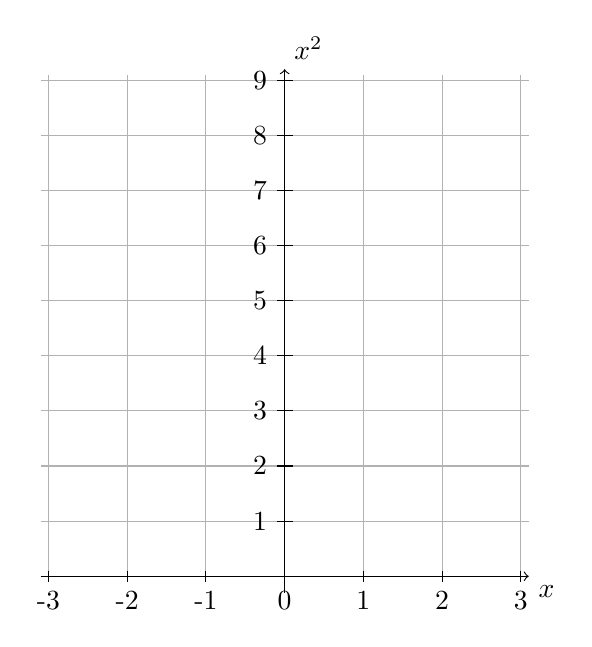
\begin{tikzpicture}[yscale=0.7]
            \draw[black!30!white] (-3.1,0) grid (3.1,9.1);
            \draw[->] (-3.1,0)--(3.1,0) node[below right] {\(x\)};
            \draw[->] (0,-0.3)--(0,9.2) node[above right] {\(x^2\)};
            \foreach \x in {-3,...,3}{
                \draw (\x, 0.1)--(\x,-0.1) node[below]{\x};
            }
            \foreach \y in {1,...,9}{
                \draw (0.1,\y)--(-0.1,\y) node[left]{\y};
            }
        \end{tikzpicture}

        Y a-t-il des symétries
    \end{exo}

    \prof{
        Enchaîner sur le cours sur la fonction carré.
    }

    \section{Utiliser la fonction carré}
    \begin{exo}
        À l'aide de la représentation graphique de la fonction carré, résoudre les équations suivantes : \begin{tasks}(3)
        \task \(x^2 = 4\)
        \task \(x^2 = 1\)
        \task \(x^2 = 0\)
        \task \(x^2 = 2\)
        \task \(x^2 = -1\)
        \task \(x^2 = 3\)
        \end{tasks}
    \end{exo}

        \begin{exo}
        À l'aide de la représentation graphique de la fonction carré, résoudre les inéquations suivantes : \begin{tasks}(3)
        \task \(x^2 \leq 4\)
        \task \(x^2 \geq 1\)
        \task \(x^2 \leq 0\)
        \task \(x^2 < 2\)
        \task \(x^2 < -1\)
        \task \(x^2 \geq -1\)
        \end{tasks}
    \end{exo}

     \begin{exo}
        Sans les calculer, dire quel est le plus grand nombre des deux \begin{tasks}(2)
        \task \(12^2\) et \(13^2\)
        \task \((-3,7)^2\) et \((-1,2)^2\)
        \task \((-2.5)^2\) et \(4,2^2\)
        \task \(2.5^2\) et \((-4,2)^2\)
        \end{tasks}
    \end{exo}

    \begin{exo}[][appro]
        \begin{enumerate}
            \item Enlever les parenthèses dans les expressions suivantes : \begin{tasks}(3)
                \task \((2x)^2\)
                \task \((-5x)^2\)
                \task \(\left(\dfrac{x}{2}\right)^2\)
            \end{tasks}
            \item Si \(a\) et \(b\) sont des nombres, peut-on enlever les parenthèses dans \((ab)^2\) ? 
            \item Écrire les nombres suivants comme un carré : \begin{tasks}(2)
                \task \(4x^2\)
                \task \(49t^2\)
                \task \(\dfrac{9}{4}y^2\)
                \task \(5a^2\)
            \end{tasks}
        \end{enumerate}
    \end{exo}

    \begin{exo}[Vrai ou faux][appro]
        
        Pour chacune des affirmations suivantes, indiquer si elle est \textbf{vraie} ou \textbf{fausse}.
        \textbf{Justifier} chaque réponse.

        \begin{tasks}
        \task $(-4)^2=-16$

        \task $(-4)^2=4^2$

        \task Si $a<0$, alors $a^2<0$.

        \task Si $a^2=25$, alors $a=5$.

        \task Si $a^2=b^2$, alors $a=b$.

        \task Si $a<b$, alors $a^2<b^2$.

        \task $(-2,5)^2=2,5^2$

        \task Pour tout nombre $x$, on a $(-x)^2=x^2$.

        \end{tasks}

    \end{exo}

    \begin{exo}[][appro]
        La distance de freinage d'un véhicule est donnée en fonction de sa vitesse par la fonction \(d(v) = 0.14v^2\) où \(v\) représente la vitesse du véhicule. 
        \begin{enumerate}
            \item Quelle est la distance parcourue après freinage si le véhicule roule à 90km/h ?
            \item Dans une ruelle, la vitesse est limitée à 30km/h. Un automobiliste imprudent roule à 10km/h au dessus de la limite de vitesse. Comment évoluera la distance de freinage par rapport à s'il roulait en règle
            \prof{
                Faut reformuler la question, je me tire une balle rien qu'à la lire
            }
        \end{enumerate}
    \end{exo}
\end{multicols}
\end{document}
